\documentclass[11pt,letterpaper]{article}

\usepackage[margin=1in]{geometry}
\usepackage[T1]{fontenc}
\usepackage[utf8]{inputenc}
\usepackage{microtype}
\usepackage{amsmath,amssymb}
\usepackage{booktabs}
\usepackage{graphicx}
\usepackage{caption}
\usepackage{authblk}
\usepackage{enumitem}
\usepackage[hyphens]{url}
\usepackage{xcolor}
\usepackage[round,authoryear]{natbib}
\usepackage{hyperref}

\hypersetup{
  pdftitle={Dual-Momentum Regime Switching under Halal Screens: An Exploratory Backtest of 12-1 Relative Strength and a 200-Day SMA Overlay, 2019-2024},
  pdfauthor={Rao Abdul Hadi},
  pdfsubject={Halal equity investing, dual momentum, absolute momentum, AAOIFI screens},
  pdfkeywords={dual momentum, relative strength, absolute momentum, AAOIFI, Sharia-compliant equities, regime switching, backtest},
  colorlinks=true,
  citecolor=blue,
  linkcolor=blue,
  urlcolor=blue
}

\captionsetup{font=small,labelfont=bf,skip=6pt}
\setlength{\parindent}{1.5em}
\setlength{\parskip}{0pt}
\setlist[itemize]{leftmargin=1.5em,itemsep=0.2em,topsep=0.35em}
\setlist[enumerate]{leftmargin=1.5em,itemsep=0.2em,topsep=0.35em}

\renewcommand\Authfont{\normalsize}
\renewcommand\Affilfont{\small}
\setlength{\affilsep}{0.6em}

\title{\textbf{Dual-Momentum Regime Switching under Halal Screens:\\
An Exploratory Backtest of 12--1 Relative Strength and a 200-Day SMA Overlay, 2019--2024}}

\author[1]{Rao Abdul Hadi\thanks{Corresponding author. Email: \href{mailto:raoabdulhadi952@gmail.com}{raoabdulhadi952@gmail.com}.}}
\affil[1]{Monterey Finance, Halal Quant Research Lab}

\date{September 2026}

\begin{document}
\maketitle

\begin{abstract}
\noindent
This paper tests a dual-momentum rule inside a Halal-screened S\&P~500 universe. After banned businesses and AAOIFI financial-ratio screens, I rank survivors by 12--1 month relative price strength versus SPY, keep the top quintile, and cap-weight the book. Absolute momentum is layered on top: when SPY closes below its 200-day simple moving average, the portfolio holds cash until the trend recovers. From 19~December~2019 through 30~December~2024 the dual-momentum book returned 18.8\% compound annual growth, against 14.8\% for the S\&P~500 (SPY) and 17.8\% for a Halal large-cap ETF (SPUS). Maximum drawdown was $-15.4\%$, roughly half the troughs of SPY ($-33.7\%$) and SPUS ($-30.8\%$). The SMA overlay is the main driver of that gap: the same momentum screen without the regime filter returned only 13.4\% CAGR with a $-30.2\%$ drawdown. Calendar years tell the same story. Dual momentum led in 2020 ($+34.4\%$) and limited 2022 losses to $-5.5\%$ while SPUS fell $-22.8\%$; it lagged SPUS in the strong bull years 2021, 2023, and 2024. Momentum quintiles inside the Halal pool are not monotonic---Q2 beat Q1---so the live edge looks more like regime timing than a clean relative-strength premium. The sample includes one clear bear year and several bull years, turnover is high, and the book remains tech-tilted. The numbers should be read as an exploratory backtest, not as a forecast or a live-return target.
\end{abstract}

\noindent\textbf{Keywords:}
dual momentum; relative strength; absolute momentum; 200-day SMA; AAOIFI; Sharia-compliant equities; regime switching; backtest.

\noindent\textbf{JEL classification:} G11, G12, Z12.

\noindent\textbf{Code:}
Replication notebook and figures are in the Monterey Finance repository,
\url{https://github.com/regional-specter/Monterey-Finance},
under \path{Research/papers/04-dual-momentum-reg-switch/}.

\section{Introduction}

Cross-sectional momentum---buying recent winners and avoiding recent losers---is one of the most studied anomalies in equity markets \citep{jegadeesh1993,asness2013}. Time-series or absolute momentum asks a separate question: whether the broad market itself is in an uptrend worth participating in \citep{moskowitz2012}. Dual momentum combines the two: rank stocks by relative strength, then stand aside when an absolute trend rule says risk is off \citep{antonacci2014}. The usual absolute filter is a long moving average on a market proxy. When price is below that average, the book holds cash (or another defensive asset) rather than the momentum basket.

Islamic equity screens change the opportunity set before either signal is applied. AAOIFI financial-ratio limits cap interest-bearing debt, cash, and receivables relative to market value, and a separate activity screen removes banks, conventional insurance, alcohol, tobacco, gambling, weapons, and similar businesses \citep{aaoifi21,derigs2008}. Those screens strip out many leveraged financials and leave a larger weight in operating businesses. The economic hope in this paper is that speculative, highly leveraged momentum turnarounds are partly filtered out before ranking, so that relative strength and the SMA overlay are applied to a cleaner Halal pool. That hope is not automatic. Screens also concentrate the universe toward technology and other growth sectors, and any backtest that looks good after 2019 may simply be riding the same mega-cap winners that dominated the sample.

The live rule tested here is therefore narrow. After banned businesses and the AAOIFI debt, cash, and receivables tests, score names by 12--1 month return relative to SPY, keep the top quintile, and cap-weight. Between rebalances, if SPY is below its 200-day simple moving average, hold cash. The question is whether that dual-momentum book improves drawdown protection against both an all-stock benchmark (SPY) and a Halal large-cap benchmark (SPUS), and whether the improvement comes from relative ranking, from the regime overlay, or from both.

It does improve headline risk-adjusted returns. The SMA overlay is what separates the live book from a plain Halal momentum sleeve that underperforms SPY. Relative-strength quintiles inside the Halal universe are not monotonic, so I treat the ranking step as a selection device rather than as proof of a clean momentum factor premium. The rest of the paper is organized as follows. Section~\ref{sec:data} describes the universe, screens, and signal definitions. Section~\ref{sec:rules} states the portfolio rules. Section~\ref{sec:results} reports live-window performance, calendar years, drawdowns, regime exposure, and the quintile diagnostic. Section~\ref{sec:attrib} looks at alpha, beta, and sector mix. Section~\ref{sec:limits} covers turnover, purification, data limits, and what would be required before treating this as a live mandate. Section~\ref{sec:conc} concludes.

\section{Data, screens, and signal definitions}
\label{sec:data}

\subsection{Universe}

The starting list is the current S\&P~500 (503 tickers). A one-time activity screen removes 64 names, leaving 439 sector-eligible stocks. Financial-ratio screens then re-run at every month-end on filings that would have been known as of that date. Fundamentals come from SEC EDGAR companyfacts when a CIK exists, otherwise from Yahoo annual statements with a 90-day publication lag. I use \texttt{filed\_date} for point-in-time filtering.

The requested price sample is 1~January~2019 through 31~December~2024, with about 15 months of earlier prices for the 12--1 lookback and the 200-day SMA. The first rebalance with holdings is 31~January~2019. Performance statistics start on the first day the strategy and both benchmarks overlap with live returns, 19~December~2019 (SPUS inception), and run through 30~December~2024 (1{,}265 trading days). Days before that aligned live date are omitted from the headline tables, not filled with zeros.

Yahoo had no in-sample price history for Q, SNDK, and FDXF. Those names are skipped where data are missing. A small set of symbols also failed a longer fundamentals price pull and are skipped on that call.

\subsection{Screening standard}

The financial screens follow AAOIFI ratios, not the Dow Jones Islamic Market (DJIM) thresholds \citep{aaoifi21,derigs2008}. The debt rule in this test is total debt below 30\% of trailing 24-month market cap, together with the library's cash and receivables screens. Compliance is a hard constraint. A name that fails on a rebalance date is not held.

SPUS (SP Funds S\&P~500 Sharia Industry Exclusions) is the Halal index comparison. It is a cap-weighted, industry-exclusion ETF. It is not identical to a pure AAOIFI financial-ratio index, so beating SPUS is not the same as beating ``the'' Sharia market. SPY is the all-stock benchmark and the regime proxy.

Table~\ref{tab:universe} summarizes the design choices.

\begin{table}[htbp]
\centering
\caption{Universe, screens, and sample.}
\label{tab:universe}
\begin{tabular}{ll}
\toprule
Item & Choice \\
\midrule
Target factors & 12--1 relative momentum; SPY vs 200-day SMA absolute trend \\
Starting universe & Current S\&P~500 list (503 tickers) \\
After banned-business screen & 439 tickers (64 removed) \\
Screening standard & AAOIFI financial ratios, not DJIM \\
Halal benchmark & SPUS (SP Funds S\&P~500 Sharia Industry Exclusions) \\
All-stock / regime proxy & SPY (S\&P~500) \\
Sample requested & 1~Jan~2019 -- 31~Dec~2024 \\
First invested rebalance & 31~Jan~2019 \\
Live window used for stats & 19~Dec~2019 -- 30~Dec~2024 (1{,}265 trading days) \\
\bottomrule
\end{tabular}
\end{table}

\subsection{Relative and absolute momentum}

Relative strength follows the classic 12--1 convention \citep{jegadeesh1993}: the trailing return over about 252 trading days, skipping the most recent 21 days to reduce short-term reversal noise. Relative momentum subtracts the same window for SPY so the book tilts toward names outperforming the broad market:
\[
\mathrm{RelMom}_{i,t}
= R_{i}(t-1\mathrm{m},\, t-12\mathrm{m})
- R_{\mathrm{SPY}}(t-1\mathrm{m},\, t-12\mathrm{m}).
\]

Absolute momentum is a daily risk-on / risk-off rule on SPY. Let $\mathrm{SMA}_{200,t}$ be the trailing 200-day simple moving average of SPY's adjusted close. The book is invested when
\[
P_{\mathrm{SPY},t} > \mathrm{SMA}_{200,t}
\]
and holds cash otherwise. That is the Antonacci absolute-momentum overlay applied to a Halal relative-strength sleeve \citep{antonacci2014,moskowitz2012}. I do not claim that AAOIFI screens create a momentum premium by themselves. The live window includes one deep risk-off year (2022) and several bull years. The no-SMA robustness sleeve is there to isolate whether the overlay, not the ranking alone, drives drawdown protection.

\section{Portfolio rules}
\label{sec:rules}

Rules are applied at month-end for selection and daily for the regime filter. There is no intra-month stop-loss and no single-name position cap beyond cap-weighting.

\subsection{Pipeline at each month-end}

\begin{enumerate}
  \item Start from the sector-eligible S\&P~500 list (439 names).
  \item Drop names that fail the AAOIFI debt, cash, or receivables screens on filings known as of that date.
  \item Score each survivor by 12--1 return relative to SPY.
  \item Keep the top quintile by relative momentum (\texttt{KEEP\_QUANTILE} $= 0.20$).
  \item Cap-weight by market cap. No equal-weight, no inverse-volatility, and no optimizer.
  \item Between rebalances, if SPY is below its 200-day SMA, hold cash at a 0\% daily return until the trend recovers.
  \item Repeat selection at month-end (\texttt{REBALANCE\_FREQ} $=$ \texttt{ME}).
\end{enumerate}

If fewer than 15 names survive (\texttt{MIN\_HOLDINGS}), that month is skipped. Cash months from a thin book are treated as missing until the first invested date. After the book is live, regime cash days are recorded as 0\% returns, not as missing.

\begin{table}[htbp]
\centering
\caption{Entry, exit, and risk limits.}
\label{tab:rules}
\small
\begin{tabular}{lp{0.62\textwidth}}
\toprule
Rule & Specification \\
\midrule
Entry & Halal, top quintile by 12--1 relative momentum vs SPY, SPY above 200-day SMA \\
Exit & Sold at the next month-end if the name fails AAOIFI or drops out of the top quintile; full book to cash when SPY $<$ 200-day SMA \\
Intra-month stop-loss & None beyond the daily SMA regime check \\
Position cap & None beyond cap-weight \\
Cash when thin & Skip the month if holdings $< 15$ \\
Robustness twin & Same momentum screen without the SMA cash rule \\
\bottomrule
\end{tabular}
\end{table}

At the last rebalance (31~December~2024), Meta was 20.8\% of the book, Broadcom 14.7\%, Walmart 9.9\%, Oracle 6.2\%, and Costco 5.5\%. That is a concentrated mega-cap winners book by construction. A 5\% or 8\% name cap would change both risk and return. I leave that for a follow-up rather than rewriting the live rule after seeing the weights.

\subsection{Holdings and regime exposure through time}

Median live book size is 47 names (minimum 43, maximum 55). At the last rebalance the funnel was roughly 429 names with fundamentals, 268 Halal, and 54 momentum picks. The strategy was invested on 80.8\% of live trading days; the rest were cash under the SMA rule.

\begin{figure}[htbp]
\centering

\includegraphics[width=0.88\textwidth]{figures/holdings-count.png}
\caption{Number of names held at each month-end. The book stays in a stable sleeve of about 45--55 names through the sample.}
\label{fig:holdings}
\end{figure}

\begin{figure}[htbp]
\centering
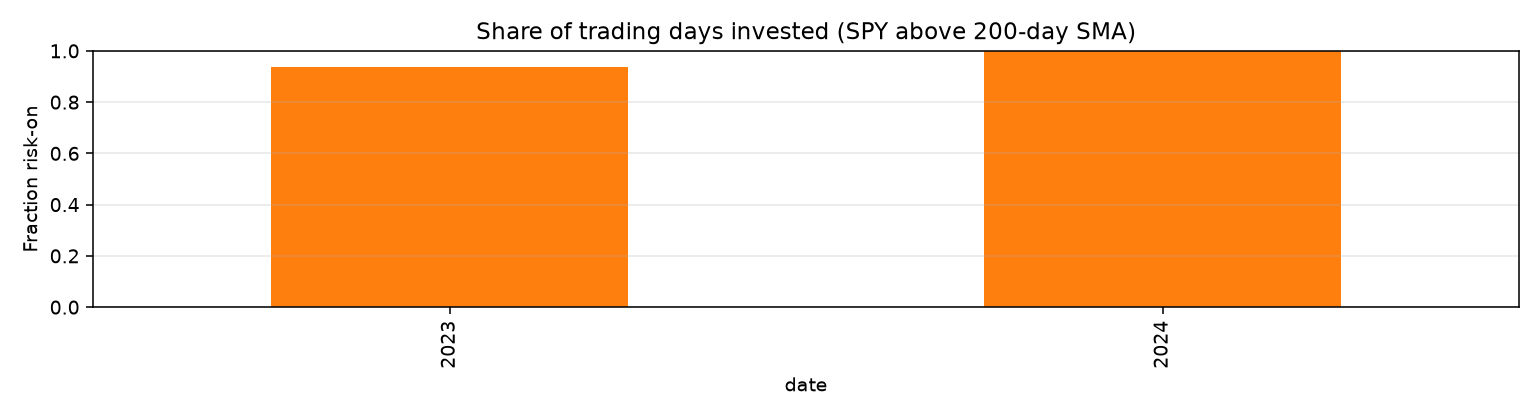
\includegraphics[width=0.88\textwidth]{figures/regime-exposure.png}
\caption{Share of trading days invested each year (SPY above its 200-day SMA). 2022 is the clear risk-off year.}
\label{fig:regime}
\end{figure}

Sharia status and relative-momentum rank are re-checked every month. A held name that fails is exited at that rebalance. The SMA filter is checked daily between rebalances.

\section{Empirical performance}
\label{sec:results}

All headline numbers use the live window only: 19~December~2019 through 30~December~2024. Sharpe and Sortino use a 2\% risk-free rate. Maximum drawdown is peak-to-trough on the growth curve.

\subsection{Headline results}

\begin{table}[htbp]
\centering
\caption{Live-window performance, 19~Dec~2019 -- 30~Dec~2024.}
\label{tab:perf}
\small
\begin{tabular}{lrrrrrr}
\toprule
Book & CAGR & Vol. & Sharpe & Sortino & Max DD & Calmar \\
\midrule
Halal dual momentum              & 18.81\% & 17.72\% & 0.95 & 1.17 & $-15.39\%$ & 1.22 \\
Momentum (no SMA filter)         & 13.38\% & 24.70\% & 0.55 & 0.71 & $-30.15\%$ & 0.44 \\
S\&P~500 (SPY)                   & 14.75\% & 20.94\% & 0.67 & 0.81 & $-33.72\%$ & 0.44 \\
Halal (SPUS)                     & 17.78\% & 21.58\% & 0.77 & 1.02 & $-30.80\%$ & 0.58 \\
\bottomrule
\end{tabular}
\end{table}

The dual-momentum book beat both benchmarks on CAGR, volatility, Sharpe, Sortino, maximum drawdown, and Calmar. The no-SMA robustness sleeve underperformed SPY on every risk-adjusted metric and took a drawdown almost as deep as SPUS. The overlay---not relative ranking alone---is what produces the live result.

These CAGRs are annualized figures from a sample that includes the 2020 crash, the 2022 bear market, and the 2023--2024 recovery. They are not a forecast of 19\% a year.

\begin{figure}[htbp]
\centering

\includegraphics[width=0.88\textwidth]{figures/equity-curves.png}
\caption{Growth of \$1 in the live window. Flat segments on the dual-momentum line are cash periods under the 200-day SMA rule.}
\label{fig:equity}
\end{figure}

\begin{figure}[htbp]
\centering

\includegraphics[width=0.88\textwidth]{figures/rolling-excess.png}
\caption{Rolling 12-month excess return versus SPY. Excess is volatile and not permanently positive.}
\label{fig:excess}
\end{figure}

\subsection{Calendar years}

\begin{table}[htbp]
\centering
\caption{Calendar-year total returns inside the live window.}
\label{tab:calendar}
\begin{tabular}{lrrr}
\toprule
Year & Halal dual momentum & S\&P~500 & Halal (SPUS) \\
\midrule
2019 & 1.25\%  & 1.21\%   & 0.81\% \\
2020 & 34.44\% & 18.33\%  & 25.68\% \\
2021 & 22.23\% & 28.73\%  & 35.62\% \\
2022 & $-5.48\%$ & $-18.18\%$ & $-22.76\%$ \\
2023 & 25.52\% & 26.18\%  & 34.20\% \\
2024 & 20.36\% & 25.34\%  & 27.67\% \\
\bottomrule
\end{tabular}
\end{table}

\begin{figure}[htbp]
\centering

\includegraphics[width=0.88\textwidth]{figures/calendar-year-returns.png}
\caption{Calendar-year returns. Dual momentum leads in 2020 and loses much less in 2022; it lags SPUS in 2021, 2023, and 2024.}
\label{fig:calendar}
\end{figure}

2019 is only a stub after SPUS inception (19~December). The economically interesting years are 2020 and 2022. Dual momentum made more in the COVID recovery and lost far less in the 2022 bear, when it was risk-on on only about one-fifth of trading days. In the strong bull years 2021, 2023, and 2024 it trailed both SPY and SPUS. That is the expected shape of a strategy that spends material time in cash.

\subsection{Drawdowns}

\begin{figure}[htbp]
\centering

\includegraphics[width=0.88\textwidth]{figures/drawdowns.png}
\caption{Drawdowns in the live window. Flat plateaus on the dual-momentum line are cash periods; SPY and SPUS keep marking to market.}
\label{fig:dd}
\end{figure}

The dual-momentum book and the benchmarks diverge most in 2022. SPY and SPUS fall toward $-25\%$ to $-35\%$. Dual momentum flattens near a shallow trough while sitting in cash. That pattern is consistent with absolute momentum, not with a defensive low-volatility equity sleeve that stays invested.

\subsection{Does higher relative momentum actually pay?}

Cap-weight five buckets by 12--1 relative momentum inside the Halal universe each month. Q1 is the highest momentum and Q5 is the lowest. These quintile books stay invested; they do not apply the SMA overlay. The cut tests whether relative ranking alone is monotonic in this screened pool.

\begin{table}[htbp]
\centering
\caption{Cap-weighted relative-momentum quintiles inside the Halal universe, live window. Q1 is highest momentum. Quintiles do not use the SMA cash rule.}
\label{tab:quintiles}
\small
\begin{tabular}{lrrrrrr}
\toprule
Bucket & CAGR & Vol. & Sharpe & Sortino & Max DD & Calmar \\
\midrule
Q1 & 15.87\% & 25.67\% & 0.62 & 0.85 & $-36.76\%$ & 0.43 \\
Q2 & 19.55\% & 20.49\% & 0.88 & 1.15 & $-30.26\%$ & 0.65 \\
Q3 & 18.69\% & 20.75\% & 0.83 & 1.02 & $-35.59\%$ & 0.53 \\
Q4 & 14.31\% & 21.32\% & 0.64 & 0.84 & $-29.39\%$ & 0.49 \\
Q5 & 14.89\% & 23.39\% & 0.63 & 0.80 & $-30.15\%$ & 0.49 \\
\bottomrule
\end{tabular}
\end{table}

The pattern is not monotonic. Q2 and Q3 beat Q1 on CAGR and on risk-adjusted metrics. The cumulative Q1 minus Q5 spread ends near 1, with a deep drawdown through 2022. In this window, relative momentum alone is a noisy sort inside the Halal pool.

\begin{figure}[htbp]
\centering

\includegraphics[width=0.88\textwidth]{figures/quintile-growth.png}
\caption{Growth of \$1 by relative-momentum quintile (always invested). Q2 leads. Q1 is not the clear winner.}
\label{fig:qgrowth}
\end{figure}

\begin{figure}[htbp]
\centering

\includegraphics[width=0.88\textwidth]{figures/quintile-spread.png}
\caption{Cumulative Q1 minus Q5 relative-momentum spread. The line is noisy and finishes near flat, not a clean stair-step premium.}
\label{fig:qspread}
\end{figure}

The live book still uses the top quintile as its selection rule, then adds the SMA overlay. The cleaner comparative evidence for that design is Table~\ref{tab:perf}: with the overlay, dual momentum dominates; without it, Halal momentum loses to SPY.

\section{Attribution}
\label{sec:attrib}

Section~\ref{sec:results} shows that the book won on risk-adjusted return. This section asks whether that win looks like stock picking or like a hidden sector bet.

\subsection{Alpha, beta, and tracking error}

Daily excess returns of the dual-momentum book are regressed on each benchmark (CAPM-style, 2\% risk-free rate). Alpha is annualized.

\begin{table}[htbp]
\centering
\caption{Halal dual momentum versus each benchmark, live window.}
\label{tab:capm}
\begin{tabular}{lrrrrr}
\toprule
Benchmark & Alpha (ann.) & Beta & $R^2$ & Tracking error & Info.\ ratio \\
\midrule
S\&P~500     & 10.89\% & 0.42 & 0.25 & 19.50\% & 0.15 \\
Halal (SPUS) & 8.85\%  & 0.48 & 0.34 & 18.32\% & 0.01 \\
\bottomrule
\end{tabular}
\end{table}

Versus both benchmarks the book has low beta and low $R^2$. That is mechanical: cash periods break co-movement with continuously invested equity indexes. Leftover annualized alpha is positive, but tracking error is large and information ratios are near zero. In other words, this is not a parallel SPUS sleeve with a small tilt. It is a regime-switched book whose path looks different from buy-and-hold Halal equity, especially in 2022.

\subsection{GICS exposure}

Average month-end weights of the cap-weighted momentum book are compared with an equal-weight basket of the Halal S\&P universe.

\begin{table}[htbp]
\centering
\caption{Average GICS sector weights. Delta is momentum book minus equal-weight Halal universe.}
\label{tab:sectors}
\small
\begin{tabular}{lrrr}
\toprule
Sector & Momentum book & Halal universe (EW) & Delta \\
\midrule
Technology                 & 37.1\% & 19.1\% & $+17.9\%$ \\
Healthcare                 & 18.6\% & 13.4\% & $+5.2\%$ \\
Communication services     & 12.6\% & 5.5\%  & $+7.2\%$ \\
Consumer cyclical          & 10.7\% & 11.6\% & $-1.0\%$ \\
Consumer defensive         & 9.7\%  & 6.4\%  & $+3.3\%$ \\
Industrials                & 6.5\%  & 14.4\% & $-7.9\%$ \\
Energy                     & 5.5\%  & 4.8\%  & $+0.7\%$ \\
Real estate                & 3.4\%  & 6.8\%  & $-3.4\%$ \\
Basic materials            & 2.7\%  & 4.6\%  & $-1.8\%$ \\
Financial services         & 2.6\%  & 6.2\%  & $-3.6\%$ \\
Utilities                  & 0.7\%  & 7.1\%  & $-6.3\%$ \\
\bottomrule
\end{tabular}
\end{table}

Technology plus communication services average about 50\% of the book when invested. Industrials and utilities are underweights. That is more growth-tilted than an equal-weight Halal universe, though less extreme than the companion ROIC-compounder backtest in this series, where technology plus communication services averaged about 82\% of weight.

\begin{figure}[htbp]
\centering

\includegraphics[width=0.88\textwidth]{figures/sector-mix.png}
\caption{GICS sector mix: momentum book versus equal-weight Halal universe. The invested book is a technology and communication overweight.}
\label{fig:sectors}
\end{figure}

\subsection{What can and cannot be isolated}

The no-SMA twin isolates the regime overlay cleanly: same Halal pool, same 12--1 ranking, same cap-weights, different only in whether cash is held when SPY is below its 200-day average. That twin loses to SPY. The live book beats SPY and SPUS. The fair reading is that absolute momentum, not relative ranking alone, produced the drawdown protection in this sample.

Without a sector-neutral twin I cannot say how much of the leftover alpha is winner selection versus extra technology exposure when the book is invested. Without a longer sample I also cannot say whether the 2022 cash period generalizes to every bear market, or whether a different SMA length would have done better or worse. The product claim that survives this paper is narrower: dual momentum under AAOIFI screens improved risk-adjusted outcomes relative to SPY and SPUS from late 2019 through 2024, and the SMA overlay was necessary for that result.

\section{Limitations and implementation friction}
\label{sec:limits}

\subsection{Turnover, slippage, and net CAGR}

Turnover is one-way: half the $\ell_1$ weight change between consecutive month-end books. Trading-cost drag assumes 10~basis points per one-way turn. Regime cash exits and re-entries are not charged separately beyond the month-end turnover series.

\begin{table}[htbp]
\centering
\caption{Implementation friction on the live dual-momentum book.}
\label{tab:friction}
\begin{tabular}{lr}
\toprule
Item & Value \\
\midrule
Rebalances with holdings              & 72 \\
Average names held                    & 48.7 \\
Annualized one-way turnover           & 401.7\% \\
Assumed cost per one-way trade        & 10~bp \\
Estimated annual trading-cost drag    & 0.40\% \\
CAGR gross of trading costs           & 18.81\% \\
CAGR net of trading costs             & 18.24\% \\
\bottomrule
\end{tabular}
\end{table}

Annualized one-way turnover above 400\% is high. Monthly top-quintile momentum rotates aggressively, and cap-weights amplify names that enter or leave the winners list. Cost drag at 10~bp is about 40~bp a year. That still leaves an 18.2\% net CAGR in this sample, but real slippage on mid-cap winners and on full cash exits could be wider. I do not model market impact, borrow, or taxes.

\begin{figure}[htbp]
\centering

\includegraphics[width=0.88\textwidth]{figures/turnover.png}
\caption{One-way turnover at each rebalance. Momentum books churn; steady-state months are still large.}
\label{fig:turnover}
\end{figure}

\subsection{Purification drag}

Impure income that may require purification is reported, not ignored. Using the library's dividend-purification helper on names that appeared in the book, there were 311 dividend events while held, and annualized purification drag is about 0.02\%. That is small next to 18.8\% CAGR. Missing interest-income tags are a gap, not evidence of zero drag.

\subsection{Point-in-time compliance}

Screens are applied at each rebalance. Failed names are sold then. There is no intra-month compliance monitor beyond the daily SMA check. Sector exclusions use the current S\&P list and current activity labels, not the 2019 membership file. That is survivorship and look-ahead in the universe, even though the filings themselves use \texttt{filed\_date}.

\subsection{Data and construction issues}

SEC companyfacts supply the long fundamental history used for AAOIFI ratios. Yahoo statements are the fallback when no CIK exists. Restatements and XBRL tag mapping are not audited here. Prices come from yfinance adjusted closes.

There is no position cap, so a handful of winners can dominate when the book is invested. The top-quintile cutoff and the 200-day SMA length were fixed before the full run. They were not optimized on a hold-out, but any dual-momentum design choice in a five-year window is still partly in-sample. The live statistics start at SPUS inception, so early-2019 strategy returns before 19~December~2019 are excluded from the headline tables.

\subsection{What this paper does not show}

There is no 2008, no rising-rate recession beyond 2022, and no hold-out after a rule freeze. Relative-momentum quintiles are not monotonic. Sector mix and mega-cap winners still matter when the book is invested. Beating SPUS with a cash overlay in a sample that contains one deep risk-off year is interesting. It is not evidence that Halal dual momentum persists across every cycle, which was the original drawdown-protection question.

\section{Conclusion}
\label{sec:conc}

A cap-weighted book of AAOIFI-screened S\&P~500 names selected by 12--1 relative momentum, and held only when SPY is above its 200-day SMA, beat SPY and SPUS from late 2019 through 2024 on both compound growth and drawdown. The more informative diagnostic is the no-SMA twin, not the quintile sort. Without the regime overlay, Halal momentum underperforms SPY. With it, the book cuts maximum drawdown roughly in half and still leads on CAGR.

The product shape is coherent enough to keep studying: Halal screens, relative-strength selection, an absolute-momentum cash rule, and cap-weighting. It is not ready to promote to a live mandate. A second paper would need a frozen rule, point-in-time S\&P membership, a position-capped or sector-neutral twin, explicit transaction costs on cash exits, and at least one more independent down year. If the capped twin still beats SPUS on Calmar after costs, the dual-momentum claim has more to stand on. If it does not, the 18.8\% CAGR in this sample is mostly the combination of a Halal winners list and one well-timed cash period in 2022.

\paragraph{Reproduction.}
Run \texttt{code.ipynb} in this paper's folder with \texttt{FAST\_MODE=False} and dates 2019-01-01 to 2024-12-31. Figures are stored alongside the notebook. The public repository is \url{https://github.com/regional-specter/Monterey-Finance}.

\bibliographystyle{plainnat}
\begin{thebibliography}{9}

\bibitem[AAOIFI(2020)]{aaoifi21}
Accounting and Auditing Organization for Islamic Financial Institutions, 2020.
\newblock Financial Paper (Shares and Bonds).
\newblock Shari'ah Standard No.~21, AAOIFI, Manama.

\bibitem[Antonacci(2014)]{antonacci2014}
Antonacci, G., 2014.
\newblock Dual Momentum Investing: An Innovative Strategy for Higher Returns with Lower Risk.
\newblock McGraw-Hill, New York.

\bibitem[Asness et~al.(2013)]{asness2013}
Asness, C.~S., Moskowitz, T.~J., Pedersen, L.~H., 2013.
\newblock Value and momentum everywhere.
\newblock Journal of Finance 68, 929--985.

\bibitem[Derigs and Marzban(2008)]{derigs2008}
Derigs, U., Marzban, S., 2008.
\newblock Review and analysis of current Shariah-compliant equity screening practices.
\newblock International Journal of Islamic and Middle Eastern Finance and Management 1, 285--303.

\bibitem[Jegadeesh and Titman(1993)]{jegadeesh1993}
Jegadeesh, N., Titman, S., 1993.
\newblock Returns to buying winners and selling losers: Implications for stock market efficiency.
\newblock Journal of Finance 48, 65--91.

\bibitem[Moskowitz et~al.(2012)]{moskowitz2012}
Moskowitz, T.~J., Ooi, Y.~H., Pedersen, L.~H., 2012.
\newblock Time series momentum.
\newblock Journal of Financial Economics 104, 228--250.

\end{thebibliography}

\end{document}
